\section{Visualizing the result}
\label{sec:visualizing-results}

Visualizing the result is essential to understand the result of the deadlock detection.
Thus, we invested time in researching different ways of achieving the same result,
with and without a local installation required to make it as user-friendly as possible.

These instructions can also be found in the
\texttt{README}\footnote{\url{https://github.com/hlisdero/cargo-check-deadlock/blob/main/README.md}}
of the repository.

\subsection{Locally}

To see the \acrshort{MIR} representation of the source code, the code can be compiled
with the corresponding flag: \Rustinline{rustc --emit=mir <path_to_source_code>}

It is important to note that the nightly toolchain may produce different \acrshort{MIR}
compared to the stable version of the compiler.
The reader is referred to Sec. \ref{sec:rust-nightly} for more information.

To graph a net in \Rustinline{.dot} format, install the \Rustinline{dot} tool
following the instructions on the GraphViz website\footnote{\url{https://graphviz.org/download/}}.

Run \Rustinline{dot -Tpng net.dot -o outfile.png}
to generate a PNG image from the resulting \Rustinline{.dot} file.

Run \Rustinline{dot -Tsvg net.dot -o outfile.svg}
to generate a SVG image from the resulting \Rustinline{.dot} file.

More information and other possible image formats can be found
in the documentation\footnote{\url{https://graphviz.org/doc/info/command.html}}.

\subsection{Online}

To see the \acrshort{MIR} representation of the source code,
the Rust Playground\footnote{\url{https://play.rust-lang.org/}} may be used.

The option ``MIR'' instead of ``Run'' must be selected in the dropdown menu.
Note that the nightly version should be used instead of the stable version of \emph{rustc}.

To graph a given DOT result,
the Graphviz Online tool\footnote{\url{https://dreampuf.github.io/GraphvizOnline/}}
offers a reliable alternative to the locally-installed tools.
Alternatives exist such as Edotor\footnote{\url{https://edotor.net/}}
or SketchViz\footnote{\url{https://sketchviz.com/new}}.

\subsection{Debugging}
\label{sec:debugging}

The program supports the verbosity flags defined in the crate
\texttt{clap\_verbosity\_flag}\footnote{\url{https://docs.rs/clap-verbosity-flag/latest/clap\_verbosity\_flag/}}.
For example, running the program with the flag \texttt{-vvv} prints debug messages
that can be useful for pinpointing which line of the \acrshort{MIR} is not being translated correctly.

The tool should then be invoked as follows:

\Rustinline{cargo check-deadlock <path_to_program>/rust_program.rs -vvv}

The model checker  \acrshort{LoLA} supports printing a ``witness path''
that shows a sequence of transition firings leading to a deadlock.
This is extremely useful when extending the translator and
the \acrshort{PN} does not match the expected result for a given program.

A convenient script named \texttt{run\_lola\_and\_print\_witness\_path.sh}
is included in the repository to print the witness path for a \texttt{.lola} file.
Fig. \ref{fig:lola-output} illustrates the result of running the script on the file
shown in Listing \ref{lst:double-lock-deadlock-mir}.

\begin{figure}[!htb]
  \centering
  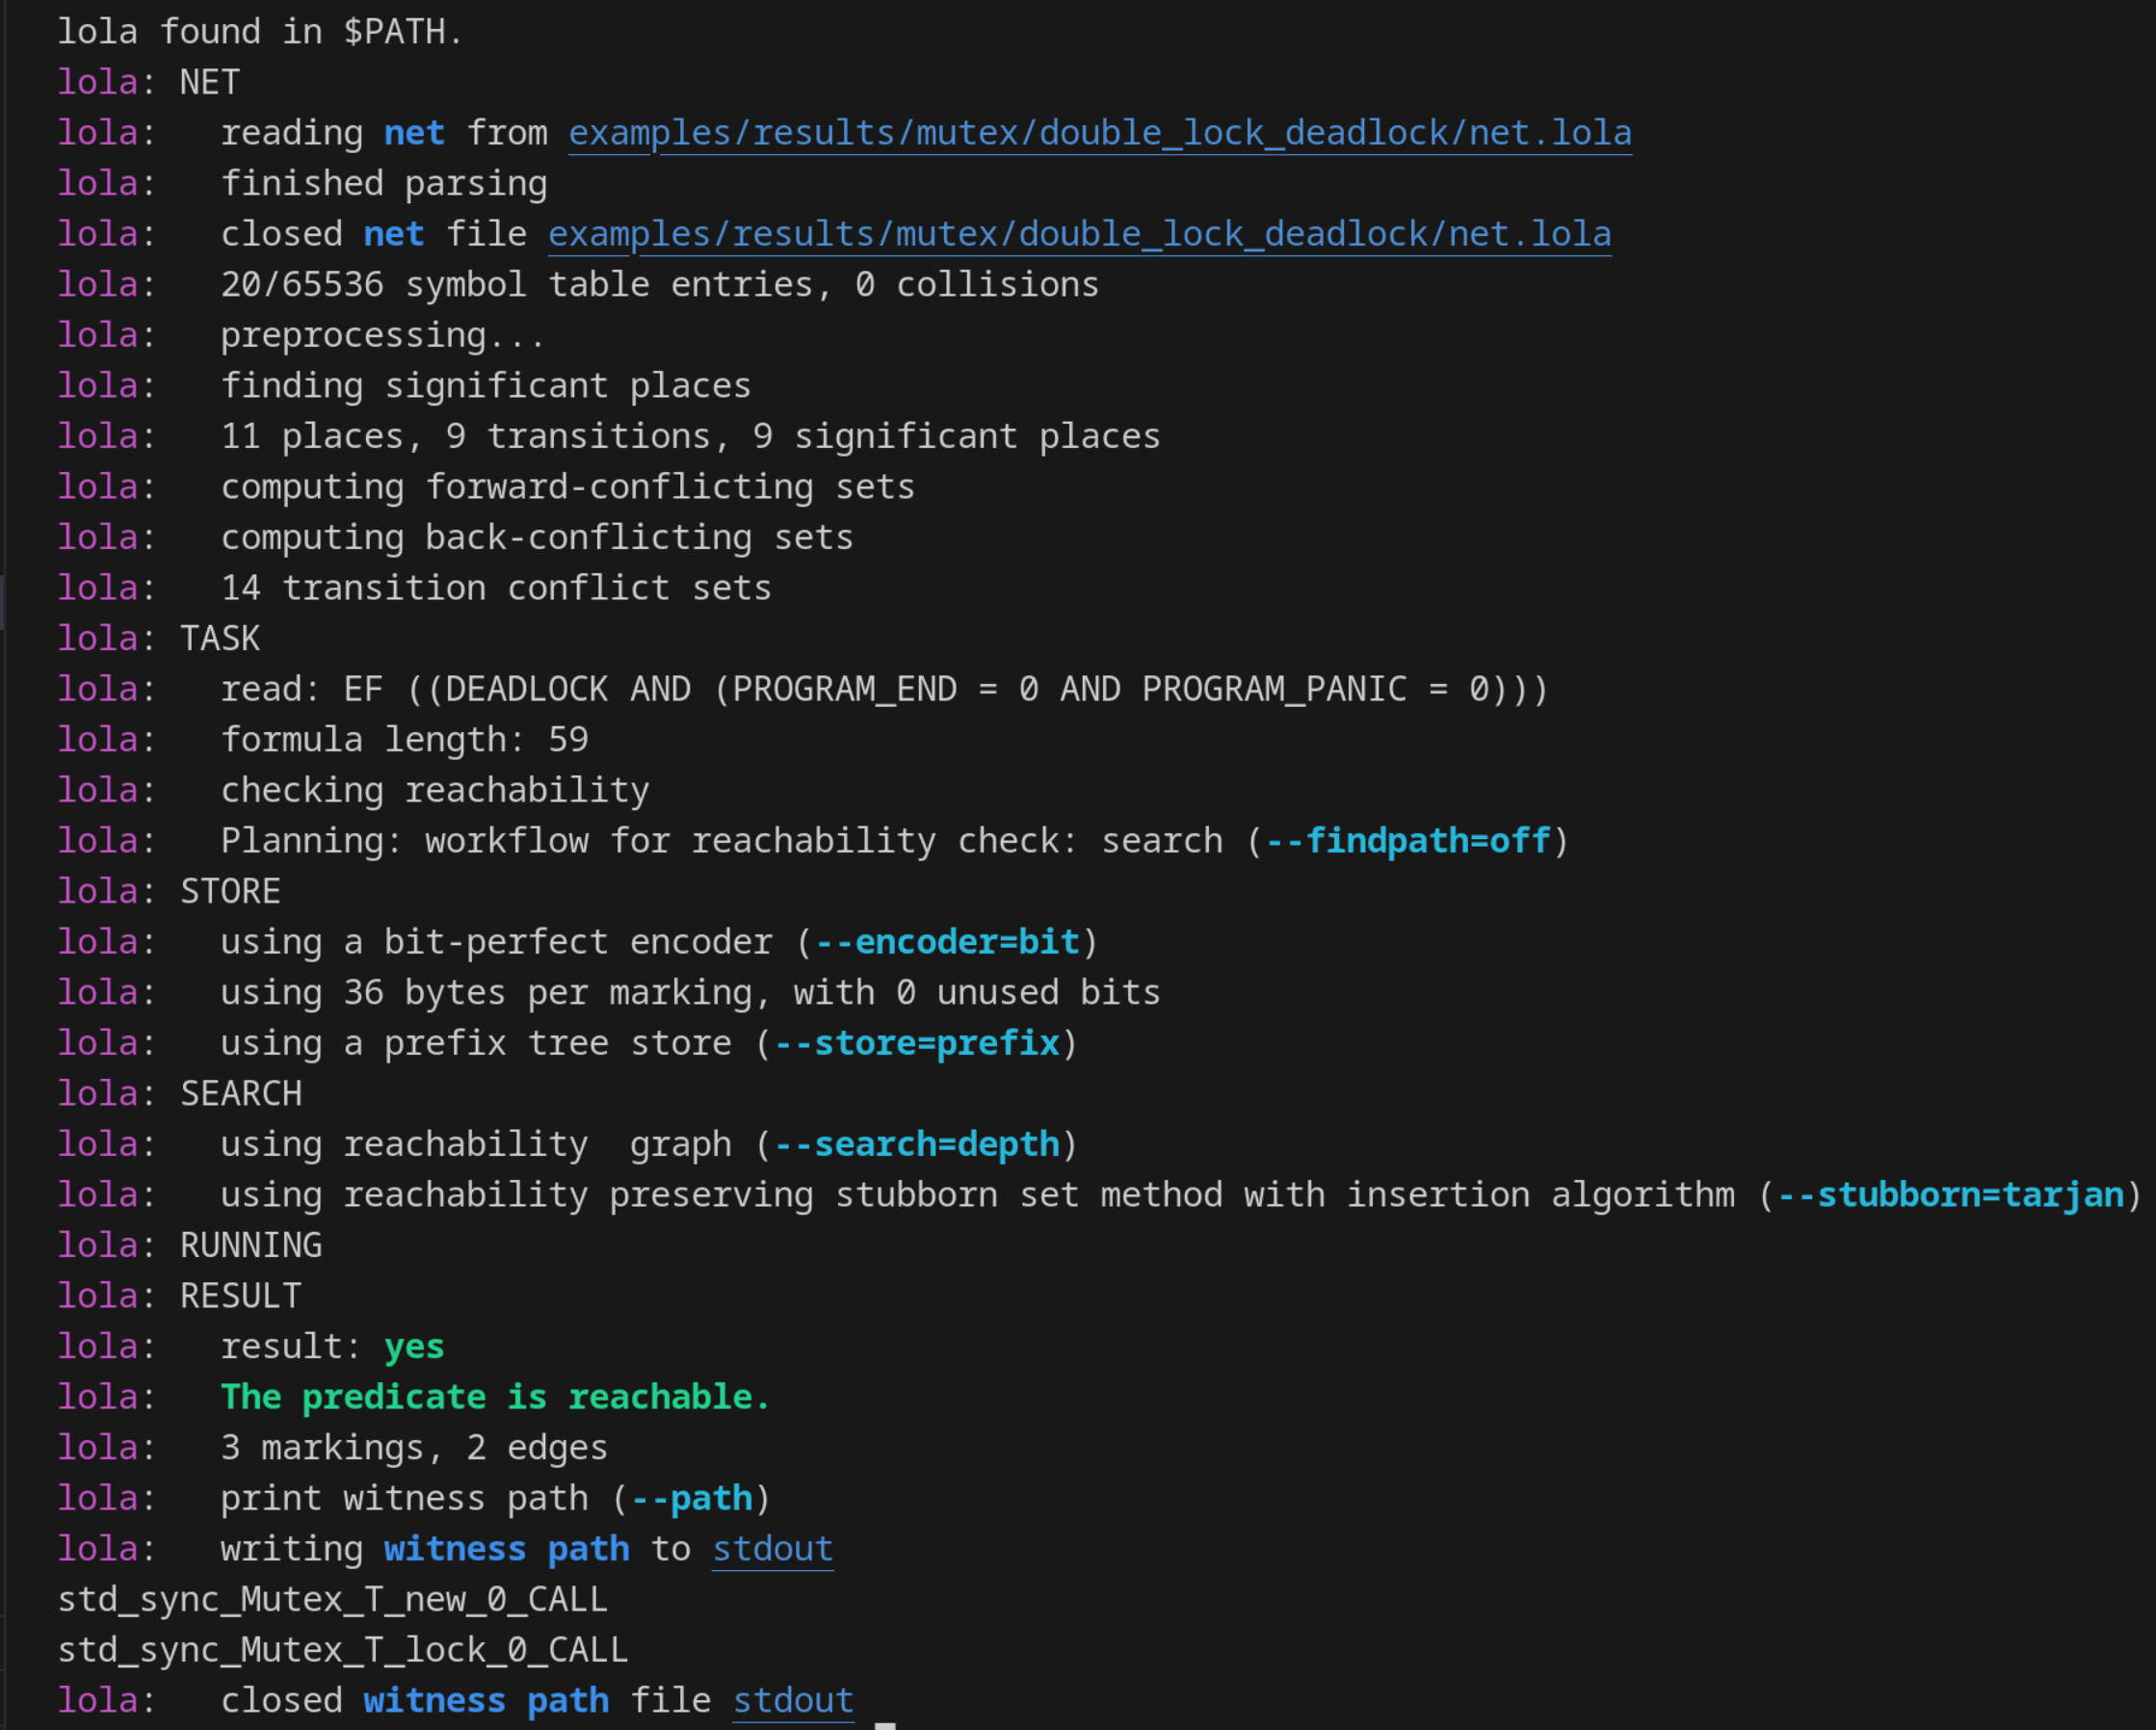
\includegraphics[width=\linewidth]{lola-output.png}
  \caption{LoLA witness path output for the program in Listing \ref{lst:double-lock-deadlock}.}
  \label{fig:lola-output}
\end{figure}